\section{Methods}



\subsection{Aggregation}
We will use Manuele Brambilla's \cite{Brambilla2013} taxonomy of collective swarm behaviors, in Figure \ref{fig:taxonomy}, to show the context for the modeled aggregation behavior. Behaviors categorized as spatially-organizing distribute robots and objects in space. These behaviors serve as fundamental building blocks for more advanced swarm behaviors, as they enable robots to connect, communicate, and interact with one another. Aggregation, the simplest of collective behaviors, groups all robots of a swarm in a region of the environment. If we assume that the robots' environment is unbounded we will have two design choices. The aggregation algorithm will either have to allow a robot to reconnect with the group or never let it disconnect from it. The first approach involves access to external information about the position of the swarm e.g. robot coordinates. The second approach relies on robots being initially connected.

% Taxonomy
\begin{figure}[H]
\caption{Taxonomy of collective swarm behaviours \cite{Brambilla2013}}
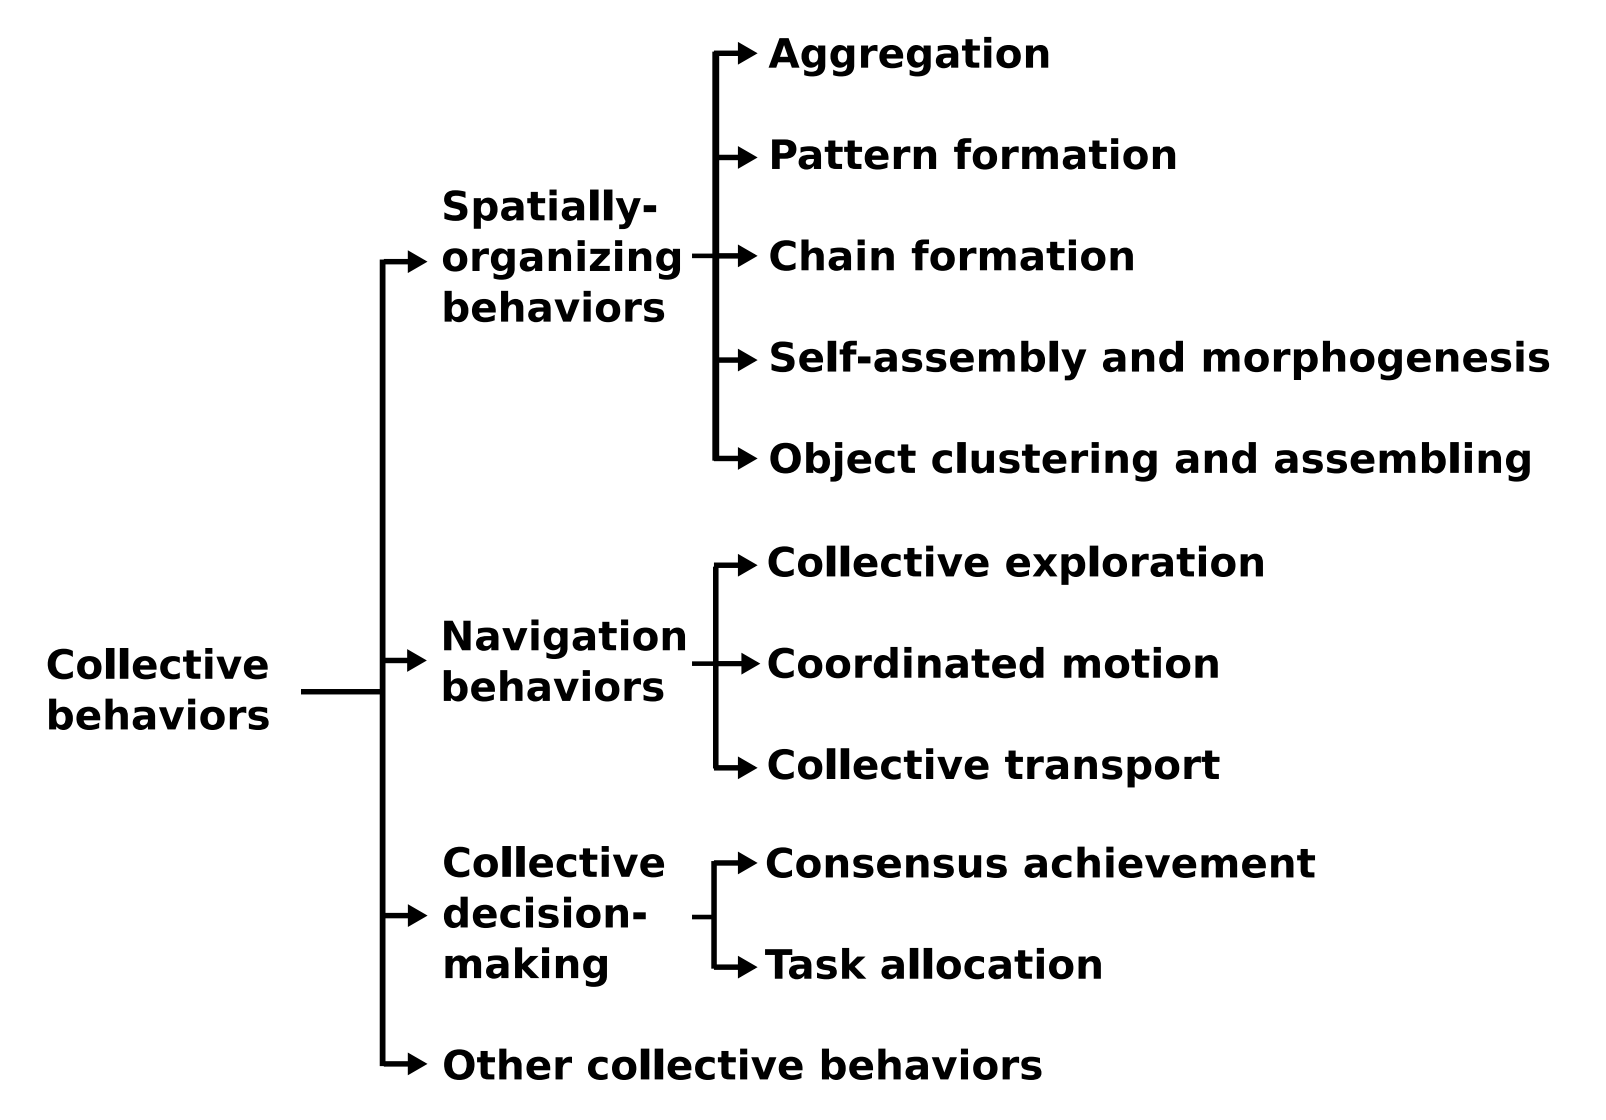
\includegraphics[width=\textwidth]{images/taxonomy.png}
\label{fig:taxonomy}
\end{figure}


\newpage
\subsection{Beta Algorithm}
The Beta algorithm is a robot swarm aggregation algorithm introduced by Julien Nembrini. It is his next iteration of the aggregation algorithm that relies on situated communication. Robots do not have information on their environment and the exact location of other robots. They are connected if they are within communication distance of the physical signal they are using. In the previous approach of the Alpha algorithm, robot movement was determined by the number of connections to other robots. In the Beta algorithm, a robot uses information about its connections as well as about connections of its connections. We will call robots that are directly connected neighbors. When losing a connection, robot will consider how many of its neighbors, are connected to the disconnected robot. If the number of neighbors that are connected to that robot is equal to or lower than the beta parameter, the robot will turn back in an attempt to reconnect. This prevents a situation previously observed in the Alpha algorithm where a single robot could disconnect from the swarm without triggering its reaction as the remaining robots would have a satisfactory number of connections. In the event of high swarm congestion, a robot will choose a random direction. Each robot keeps a list of currently and previously connected robots. Every robot can access its neighbors` current list of connections. The underlying assumption is that connected robots can exchange information. Additionally, a robot does not need to be aware of its direction. As long as it can perform a 180-degree turn and a random turn, it can move. Although the robots are unaware of their positions and environment, the algorithm will prevent them from disconnecting.

% Pseudo-code for Beta algorithm
\begin{figure}
\caption{Pseudo-code for Beta algorithm \cite{Nembrini2002}}
\begin{lstlisting}[style=code]
Create list of neighbours for robot, Nlist
k = number of neighbours in Nlist
i = 0

loop forever {
	i = i modulo cadence

	if (i = 0) {
		Send ID message

		Save copy of k in LastK
		Set reaction indicator Back to FALSE
		k = number of neighbours in Nlist
		Create LostList comparing Nlist and OldList

		for (each robot in LostList) {
			Find nShared, number of shared neighbours
			if (nShared <= beta) {
				Set reaction indicator Back to TRUE
			}
		}

		if (Back = TRUE) {
			turn robot through 180 degrees
		}
		else if (k > LastK) {
			make random turn
		}
		
		Save copy of Nlist in Oldlist
	}
	Steer the robot according to state
	Listen for calls from robots in range
	Grow Nlist with neighbours IDs and connection info

	i++
}
\end{lstlisting}
\label{fig:pseudocode}
\end{figure}



\subsection{Movement}
From the pseudocode and textual description of the Beta algorithm, we know that a robot must be able to move forward, turn 180 degrees, and make a random turn. We assume that a random turn is a turn by a random number of degrees. As the robots in a swarm should be uniform, we assume they move forward by a unit step. Because we will be focusing on verification there is a need to make some arbitrary decisions that limit the state space. We aim for limitations that will not fundamentally change the algorithm itself. The first thing to be limited is the choice of the direction a robot can move. We will limit the choice to four directions, namely, up, down, left, and right. To preserve the randomness of the turn, one of four directions is chosen at random. We assume that our source of randomness produces uniformly distributed results making all directions equally likely to draw. This means that after a random turn, there is a 75\% chance of changing direction and a 25\% chance of maintaining a current one. 

The next arbitrary decision we must make to limit the state space for verification purposes is to introduce boundaries in the environment. Robots move in four directions, a unit step at a time. The environment is a grid with points that can be occupied by robots. As the chances of movement in each direction are equal, the shape of the environment should reflect that and be a square. Whether we make a robot turn around when reaching the boundary or introduce a wrap-around mechanism, we want the influence of the boundary to be reflected equally in both horizontal and vertical directions. In our case, a robot reaching the boundary of the environment will turn 180 degrees. Our approach is suitable for modeling two-dimensional environments. The wrap-around mechanism would be more suitable if the robots were to operate on the sphere. In such a case it could be expected for two robots moving away from each other to connect. This is not the expected behavior in a two-dimensional environment.

The last simplification is made to prevent further algorithm modification. The algorithm assumes that robots are unaware of other robots' positions. A robot knows whether it is connected to the other robot but is not aware of its own or its neighbor's coordinates. As the robots can occupy a limited number of points in the bounded environment, there might occur a situation where two robots occupy the same space. We accept that situation for the following reasons. Implementing the collision-avoiding mechanism would lead to significant changes in the algorithm. Our goal is verification of the algorithm so we would like to introduce as few changes as possible. Additionally, it would be hard to estimate the influence of the collision-avoiding mechanism on the algorithm's effectiveness. Lastly, this simplification is acceptable if we assume that robots can be positioned very close to each other.



\subsection{Connection}
The algorithm assumes that robots use a range-limited omnidirectional signal that enables two-way communication. Each robot broadcasts its ID to inform other robots of its presence. If a robot receives an ID from another robot, they are within the physical range of the signal and are therefore connected. In our case, the environment is two-dimensional, and the physical signal is modeled as a circle centered at the robot's position. All robots within that circle are considered neighbors. The range of the signal is parameterized by the radius length. The radius should be larger than a unit step to allow movement but smaller than the side of the grid to keep it range-limited relative to the dimensions of the environment.

Since we are not dealing with physical robots, we have to mimic the physical signal programmatically. To achieve this we need information about robot coordinates and the radius of the physical signal. Robots are unaware of their own and their neighbor's coordinates. However, robot coordinates are stored and utilized. To determine if two robots are connected, we determine whether the Euclidean distance between their positions is smaller than the radius of their signal. Each robot keeps information about the current and previous number of connections. They also store lists of currently and previously connected robots. By comparing these lists, a robot can track the lost connections. A list of currently connected robots can be accessed by every neighboring robot. This allows a robot to determine how many of its neighbors are still connected to each of its lost connections. If the number of such neighbors is smaller or equal to the beta parameter, a robot will turn back in an attempt to reconnect.


\subsection{System variables}
To describe a robot swarm implementing the Beta algorithm we must define the minimal set of variables. The first variable is the number of robots that constitute the swarm. It has the highest influence on the resulting size of the state space. It also limits the beta parameter, as each robot can be connected to at most every other robot, excluding itself. The second most important parameter is the beta parameter. The assumption of the algorithm is that a beta equal to two guarantees coherence. This means that verification should be performed for swarms of three or more robots. Although it is assumed that robots' environment is unbounded we must limit it to make verification feasible. Environment is a square defined by the length of its side. Each robot moves in the environment a unit step at a time. It is important that the length of the unit step is relatively small in regard to the size of the environment. If the unit step size is too big we will verify the version of the algorithm where robot interaction will be greatly influenced by reaching the boundary of the environment which is an introduced limitation. The last variable that we have to define is the radius of the physical signal that we are simulating. The radius is related to both the environment size and the unit step. If we make the radius of the signal smaller or equal to the unit step size, we will promote swarm concentration. On the other side, if we make the radius of the signal bigger, we will promote swarm exploration. The upper limit on the radius of the signal is the size of the environment, we never want the signal of a robot to cover the whole environment. This would lead to a situation where a swarm is fully connected and unable to disconnect. Such configuration would lead to untruthful verification of the algorithm as most of its scenarios would not be reachable.



\subsection{Automaton}

% Automaton
\begin{figure}[H]
\caption{Timed automaton for the Beta algorithm}
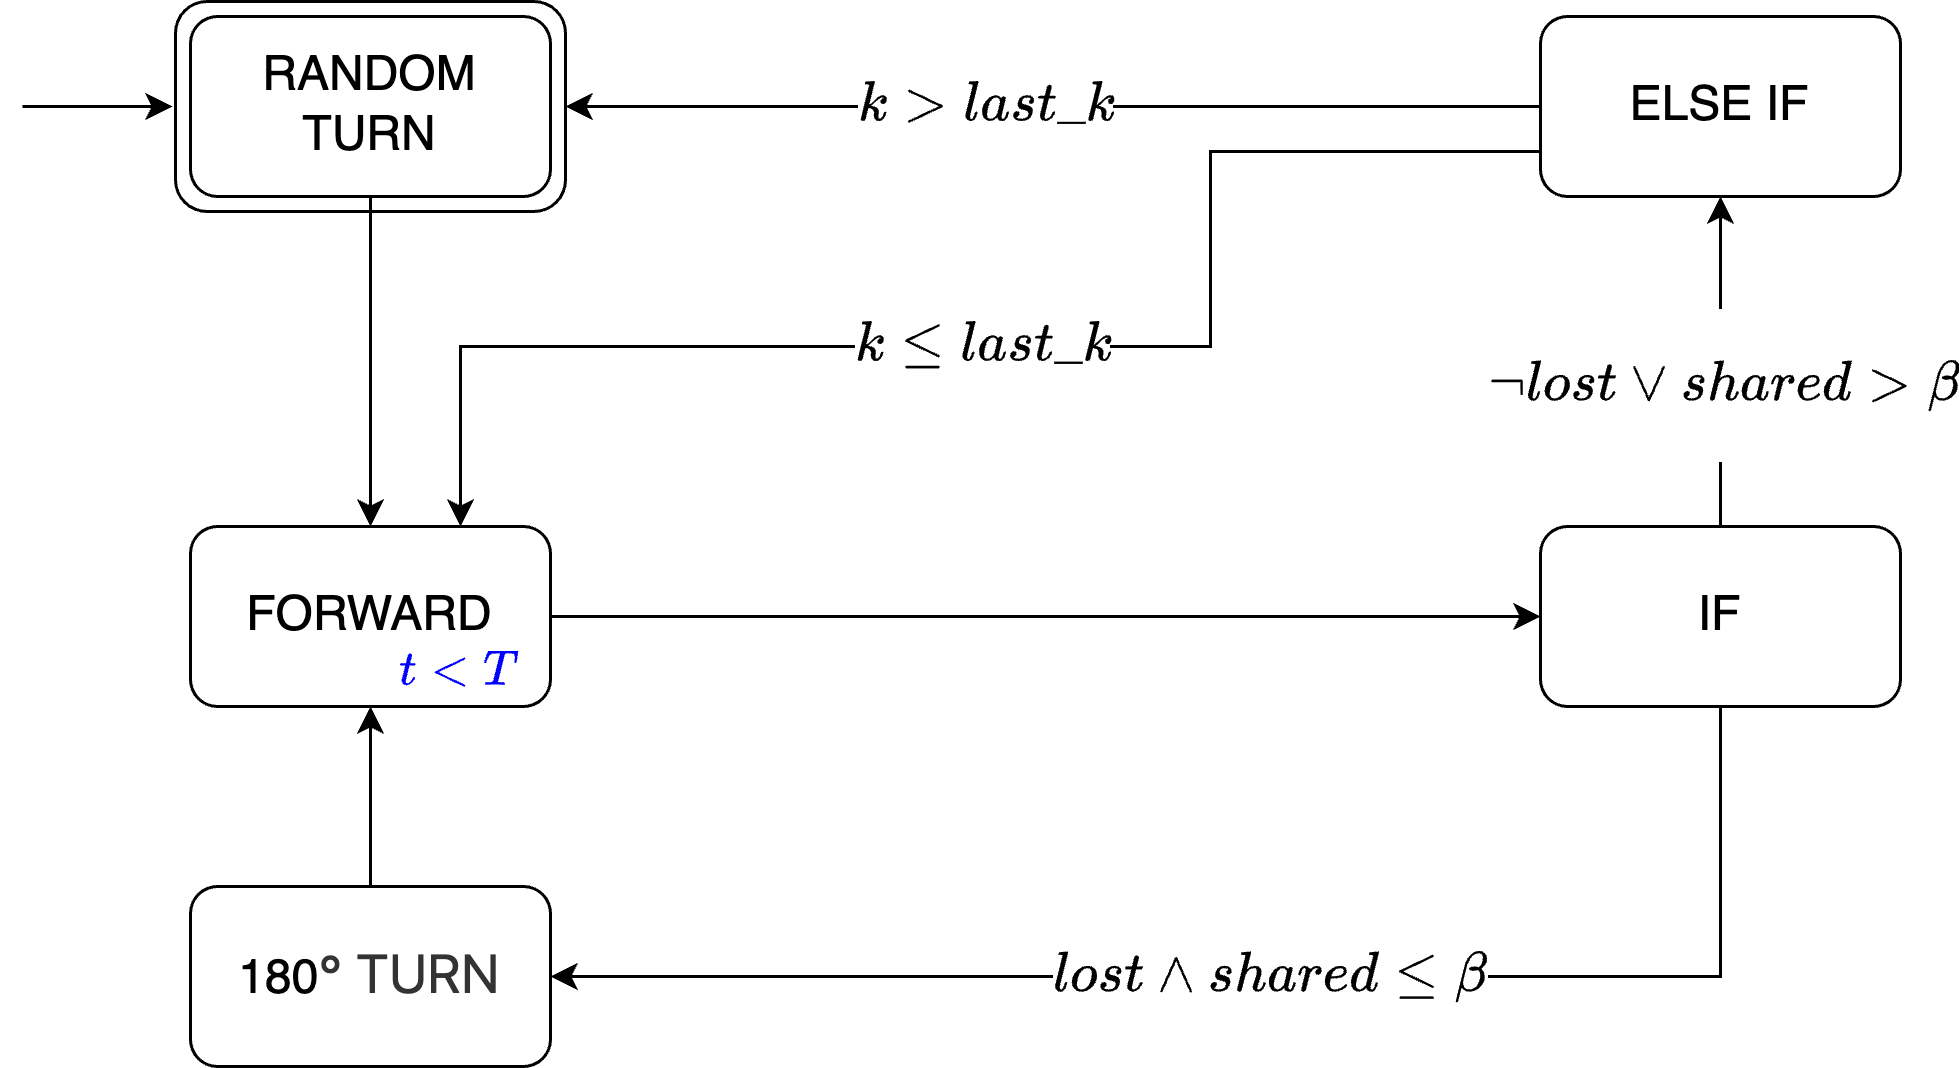
\includegraphics[width=\textwidth]{images/beta.png}
\label{fig:automaton}
\end{figure}
